\documentclass[a4paper,oneside,12pt]{extreport}

\usepackage{mmap}
\usepackage[T2A]{fontenc}
\usepackage[utf8]{inputenc}
\usepackage[english,russian]{babel}


% Текст отчёта следует печатать, соблюдая следующие размеры полей:
% левое — 30 мм, правое — 15 мм, верхнее и нижнее — 20 мм.
\usepackage[left=20mm, right=15mm, top=15mm, bottom=15mm]{geometry}

% \setlength{\parindent}{1.25cm} % Абзацный отступ

\usepackage{setspace}
%\onehalfspacing % Полуторный интервал

\frenchspacing % Равномерные пробелы
\usepackage{indentfirst} % Красная строка

\usepackage{microtype}
\sloppy

\usepackage{titlesec}
\titlespacing*{\chapter}{0pt}{-30pt}{8pt}
\titlespacing*{\section}{\parindent}{*4}{*4}
\titlespacing*{\subsection}{\parindent}{*4}{*4}
\titleformat{\chapter}{\LARGE\bfseries}{\thechapter}{20pt}{\LARGE\bfseries}
\titleformat{\section}{\Large\bfseries}{\thesection}{40pt}{\Large\bfseries}

\usepackage{graphicx}
\usepackage{caption}

\usepackage[unicode,pdftex]{hyperref}
\hypersetup{hidelinks}

%% title begin
\usepackage{wrapfig}

\makeatletter
	\def\vhrulefill#1{\leavevmode\leaders\hrule\@height#1\hfill \kern\z@}
\makeatother
%% title end

%% begin code
\usepackage{listings}
\usepackage{xcolor}

\lstset{
	basicstyle=\footnotesize\ttfamily,
	breakatwhitespace=true,
	breaklines=true,
	commentstyle=\color{gray},
	frame=single,
	keywordstyle=\color{blue},
	stringstyle=\color{red},
	tabsize=8
}

\lstdefinestyle{lispinline}{
	frame=none,
	language=Lisp
}

\newcommand{\code}[1]{\texttt{#1}}
%% end code

%% begin theorem
\usepackage{amsthm}

\makeatletter
\newtheoremstyle{indented}
	{}% measure of space to leave above the theorem
	{}% measure of space to leave below the theorem
	{}% name of font to use in the body of the theorem
	{\parindent}% measure of space to indent
	{\bfseries}% name of head font
	{.}% punctuation between head and body
	{ }% space after theorem head; " " = normal interword space
	{}% header specification (empty for default)
\makeatother

\theoremstyle{indented}

\newtheorem{definition}{Определение}[section]
\newtheorem{example}{Пример}[section]
\newtheorem{theorem}{Теорема}[section]
\newtheorem{task}{Задание}

\makeatletter
\DeclareRobustCommand\bfseriesitshape{%
	\not@math@alphabet\itshapebfseries\relax
	\fontseries\bfdefault
	\fontshape\itdefault
	\selectfont
}
\makeatother

\DeclareTextFontCommand{\textbfit}{\bfseriesitshape}
\DeclareTextFontCommand{\define}{\bfseriesitshape}
%% end theorem

%% begin columns
\usepackage{etoolbox,refcount}
\usepackage{multicol}

\newcounter{countitems}
\newcounter{nextitemizecount}
\newcommand{\setupcountitems}{%
	\stepcounter{nextitemizecount}%
	\setcounter{countitems}{0}%
	\preto\item{\stepcounter{countitems}}%
}
\makeatletter
\newcommand{\computecountitems}{%
	\edef\@currentlabel{\number\c@countitems}%
	\label{countitems@\number\numexpr\value{nextitemizecount}-1\relax}%
}
\newcommand{\nextitemizecount}{%
	\getrefnumber{countitems@\number\c@nextitemizecount}%
}
\newcommand{\previtemizecount}{%
	\getrefnumber{countitems@\number\numexpr\value{nextitemizecount}-1\relax}%
}
\makeatother
\newenvironment{AutoMultiColItemize}{%
	\ifnumcomp{\nextitemizecount}{>}{3}{\begin{multicols}{2}}{}%
		\setupcountitems\begin{itemize}}%
		{\end{itemize}%
		\unskip\computecountitems\ifnumcomp{\previtemizecount}{>}{3}{\end{multicols}}{}}
\makeatother
\newenvironment{AutoMultiColEnumerate}{%
	\ifnumcomp{\nextitemizecount}{>}{3}{\begin{multicols}{2}}{}%
		\setupcountitems\begin{enumerate}}%
		{\end{enumerate}%
		\unskip\computecountitems\ifnumcomp{\previtemizecount}{>}{3}{\end{multicols}}{}}
%% end columns



\begin{document}

\begin{titlepage}
	{\large % 14pt instead of 12pt
	\onehalfspacing
	\centering

	\begin{wrapfigure}[7]{l}{0.14\linewidth}
		\vspace{3mm}
		\hspace{-10mm}
		
\includegraphics[width=\linewidth]{img/b_logo}
		% \includegraphics[width=0.93\linewidth]{inc/img/bmstu-logo}
	\end{wrapfigure}
	{\singlespacing \footnotesize \bfseries Министерство науки и высшего образования Российской Федерации\\Федеральное государственное бюджетное образовательное учреждение\\высшего образования\\<<Московский государственный технический университет\\имени Н.~Э.~Баумана\\ (национальный исследовательский университет)>>\\(МГТУ им. Н.~Э.~Баумана)\\}

	\vspace{-2.2mm}
	\vhrulefill{0.9mm}\\
	\vspace{-7.5mm}
	\vhrulefill{0.2mm}\\
	\vspace{2mm}

	{\doublespacing \small \raggedright ФАКУЛЬТЕТ \hspace{5mm} \underline{«Информатика и системы управления»}\\
	КАФЕДРА \hspace{10mm} \underline{«Программное обеспечение ЭВМ и информационные технологии»}\\}

	\vspace{20mm}

	\begin{center}
		\noindent\begin{minipage}{1.2\textwidth}\centering
			\textbf{ОТЧЕТ ПО ЛАБОРАТОРНОЙ РАБОТЕ №18,19}\newline
			\textbf{По курсу: "Функциональное и Логическое программирование"}\newline\newline\newline
		\end{minipage}
	\end{center}

	\vspace{20mm}

	\noindent ~~Тема \underline{~~~~~~~~~~~~~~~~~~~~~~~~~~Рекурсия в прологе.~~~~~~~~~~~~~~~~~~~~~~~~~~~~~~~~~~~~~~~~~~~}\newline
	\noindent ~~Группа \underline{~~~~~~~~~~~~~~~~~~~~~~~~~~~~~~~~~~~ИУ7-63Б~~~~~~~~~~~~~~~~~~~~~~~~~~~~~~~~~~~~~~~~~~~~~~~~~}\newline
	\noindent ~~Студент \underline{~~~~~~~~~~~~~~~~~~~~~~~~~~~~Сукочева А.~~~~~~~~~~~~~~~~~~~~~~~~~~~~~~~~~~~~~~~~~~~~~~~~~~}\newline
	\noindent ~~Преподаватель \underline{~~~~~~~~~~~~~~~~~Толпинская Н.Б.~~~~~~~~~~~~~~~~~~~~~~~~~~~~~~~~~~~~~~~~~~~~~}\newline
	\noindent ~~Преподаватель \underline{~~~~~~~~~~~~~~~~~~Строганов Ю. В.~~~~~~~~~~~~~~~~~~~~~~~~~~~~~~~~~~~~~~~~~~~~}\newline


	\begin{center}
		\vfill
		Москва~---~\the\year
		~г.
	\end{center}
	}



\end{titlepage}

\setcounter{page}{2}

\section*{Практическая часть л.р.16}

\begin{task}
    Используя хвостовую рекурсию, разработать программу, позволяющую найти:

    \begin{enumerate}
        \item факториал числа;
        \item n-ое число Фибоначчи.
    \end{enumerate}

    \begin{lstlisting}[language=Prolog]
DOMAINS 
	number = integer

PREDICATES
	factorial(number, number, number).
	factorialWrapper(number, number).
	
CLAUSES
	factorial(0, Res, Res) :- !.
	factorial(Number, Current, Res) :- 
		NextNumber = Number - 1,
		Mult = Current * Number,
		factorial(NextNumber, Mult, Res).
	
	factorialWrapper(Number, -1) :- Number < 0, !. % Error. 
	factorialWrapper(Number, Res) :- factorial(Number, 1, Res).
	
GOAL
	% factorialWrapper(5, Result).
	% factorialWrapper(-5, Result).	
	factorialWrapper(0, Result).
\end{lstlisting}

    \newpage

    \begin{figure}[ht!]
    \centering{
        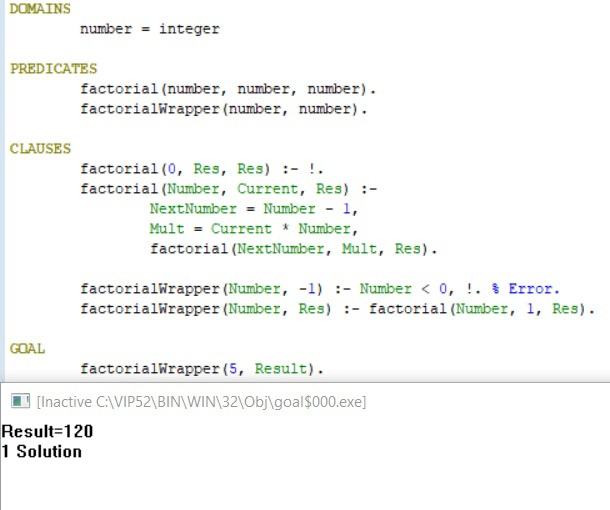
\includegraphics[width=0.9\textwidth]{img/res_lab_18/1.jpg}
        \caption{Факториал числа}}
    \end{figure}

    \begin{figure}[ht!]
        \centering{
            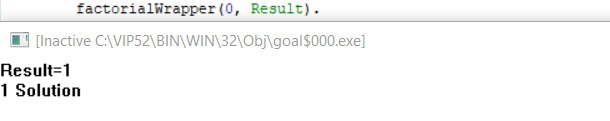
\includegraphics[width=0.9\textwidth]{img/res_lab_18/2.jpg}
            \caption{Факториал числа}}
    \end{figure}

    \begin{figure}[ht!]
    \centering{
        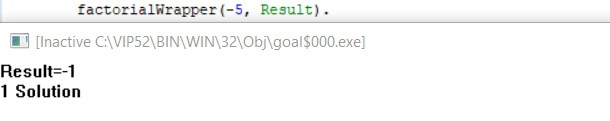
\includegraphics[width=0.9\textwidth]{img/res_lab_18/3.jpg}
        \caption{Факториал числа}}
    \end{figure}
    
    \begin{figure}[ht!]
        \centering{
            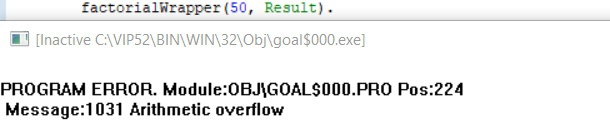
\includegraphics[width=0.9\textwidth]{img/res_lab_18/4.jpg}
            \caption{Факториал числа}}
    \end{figure}

    \newpage

    \begin{lstlisting}[language=Prolog]
DOMAINS 
	number = integer

PREDICATES
	fibonacci(number, number, number, number).
	fibonacciWrapper(number, number).

CLAUSES
	fibonacci(1, Prev, _, Prev) :- !.
	fibonacci(Number, Prev, Current, Res) :-
		NewNumber = Number - 1,
		Newprev = Current,
		NewCurrent = Prev + Current,
		fibonacci(NewNumber, NewPrev, NewCurrent, Res).
	
	
	fibonacciWrapper(Number, -1) :- Number < 1, !. % Error.
	fibonacciWrapper(Number, Res) :- fibonacci(Number, 1, 1, Res).
	
	
GOAL
	% fibonacciWrapper(-15, Result).
	% fibonacciWrapper(1, Result).
	% fibonacciWrapper(2, Result).
	% fibonacciWrapper(3, Result).
	fibonacciWrapper(8, Result).
    \end{lstlisting}

    \begin{figure}[ht!]
    \centering{
        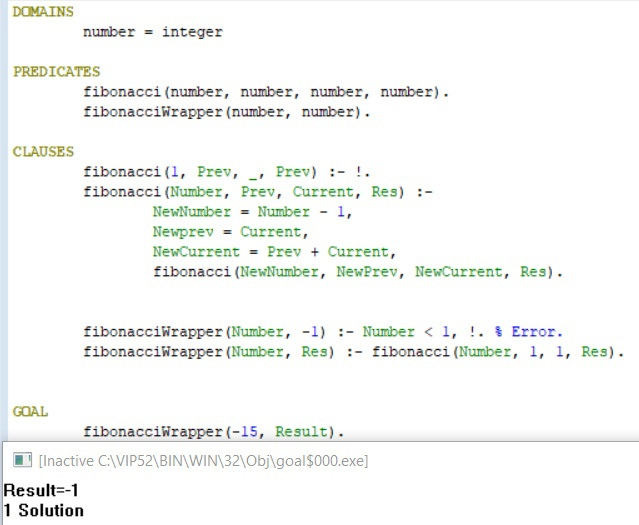
\includegraphics[width=0.9\textwidth]{img/res_lab_18/5.jpg}
        \caption{Фибоначчи}}
    \end{figure}
    
    \begin{figure}[ht!]
        \centering{
            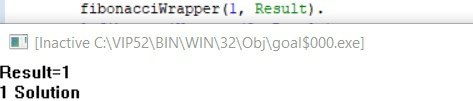
\includegraphics[width=0.9\textwidth]{img/res_lab_18/6.jpg}
            \caption{Фибоначчи}}
    \end{figure}

    \begin{figure}[ht!]
        \centering{
            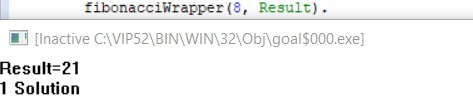
\includegraphics[width=0.9\textwidth]{img/res_lab_18/7.jpg}
            \caption{Фибоначчи}}
    \end{figure}

\end{task}

\newpage

\section*{Практическая часть л.р.17}

\begin{task}
    Используя хвостовую рекурсию, разработать эффективную программу, позволяющую:

    \begin{enumerate}
        \item найти длину списка (по верхнему уровню);
        \item найти сумму элементов числового списка;
        \item найти сумму элементов числового списка, стоящих на нечетных позициях
        исходного списка (нумерация от 0).
    \end{enumerate}

    Убедиться в правильности результатов.

    Длина списка.
    \begin{lstlisting}[language=Prolog]
DOMAINS
    list = integer*.

PREDICATES
    length(list, integer, integer).
    lengthWapper(list, integer).
    
CLAUSES
    length([], Res, Res) :- !.
    length([_|T], CurrValue, Res) :- 
        NewCurrValue = CurrValue + 1,
        length(T, NewCurrValue, Res). 
    
    lengthWapper(L, Res) :- length(L, 0, Res).

GOAL
    % lengthWapper([1, 2, 3], Result).
    % lengthWapper([], Result).
    lengthWapper([1, 2, 3, 1, 2, 3, 1, 2, 3], Result).
    \end{lstlisting}

    Сумма элементов числового списка.
    \begin{lstlisting}[language=Prolog]
DOMAINS
    list = integer*.

PREDICATES
    sum(list, integer, integer).
    sumWapper(list, integer).
    
CLAUSES
    sum([], Res, Res) :- !.
    sum([H|T], CurrValue, Res) :- 
        NewCurrValue = CurrValue + H,
        sum(T, NewCurrValue, Res). 
    
    sumWapper(L, Res) :- sum(L, 0, Res).

GOAL
    % sumWapper([1, 2, 3], Result).
    % sumWapper([], Result).
    sumWapper([1, 2, 3, 1, 2, 3, 1, 2, 3], Result).
    \end{lstlisting}

    \newpage
    
    Сумма элементов числового списка, стоящих на нечетных позициях.
    \begin{lstlisting}[language=Prolog]
DOMAINS
    list = integer*.
    flag = integer. 

PREDICATES
    sum_odd(list, integer, integer, flag).
    sum_oddWapper(list, integer).
    
CLAUSES
    sum_odd([], Res, Res, _) :- !.
    sum_odd([_|T], CurrValue, Res, 0) :- sum_odd(T, CurrValue, Res, 1).
    
    sum_odd([H|T], CurrValue, Res, 1) :- 
        NewCurrValue = CurrValue + H,
        sum_odd(T, NewCurrValue, Res, 0).
    
    sum_oddWapper(L, Res) :- sum_odd(L, 0, Res, 0). 

GOAL
    % sum_oddWapper([1, 2, 3], Result).
    %sum_oddWapper([], Result).
    %sum_oddWapper([1, 2, 3, 1, 2, 3, 1, 2, 3], Result).
    sum_oddWapper([1, 2, 3, 4, 5], Result).
    %sum_oddWapper([1], Result).
    \end{lstlisting}

    \begin{figure}[ht!]
    \centering{
        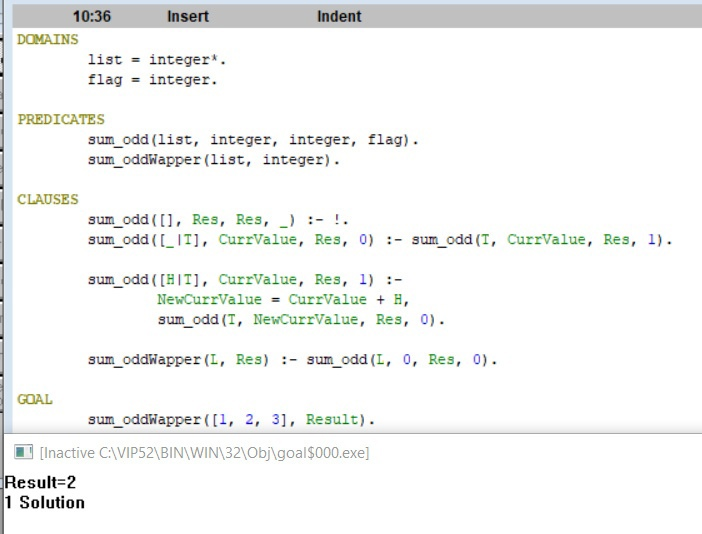
\includegraphics[width=0.9\textwidth]{img/res_lab_19/1.jpg}
        \caption{Сумма элементов числового списка, стоящих на нечетных позициях.}}
    \end{figure}
    
    \begin{figure}[ht!]
        \centering{
            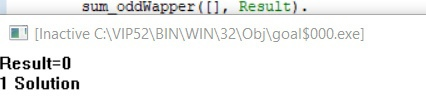
\includegraphics[width=0.9\textwidth]{img/res_lab_19/2.jpg}
            \caption{Сумма элементов числового списка, стоящих на нечетных позициях.}}
    \end{figure}

    \begin{figure}[ht!]
        \centering{
            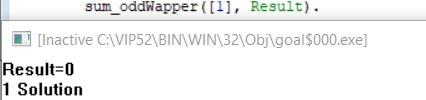
\includegraphics[width=0.9\textwidth]{img/res_lab_19/3.jpg}
            \caption{Сумма элементов числового списка, стоящих на нечетных позициях.}}
    \end{figure}
\end{task}

\newpage


\end{document}